%% ----------------------------------------------------------------
%% Results.tex
%% 2336
%% ---------------------------------------------------------------- 
\chapter{Results \& Discussion} \label{Chapter: Results}

% Parameters are defined in Results (not in Methods)
% Report is a presentation of the final results, not the whole process.
% Draw inferences from proofs

% Check that your paper is focused. Choose the point of the paper and its essential conclusion before you begin writing, stick to your choices, and write the paper so that the reader gets the point already in the abstract and the introduction. Leave out results that are not required for supporting the critical conclusion, or safely tuck them away in the supplementary information document. When editing, if you feel that your paper loses its focus at some point, take a step back and do a significant rewrite.

% Check that there is a clear question and a clear answer —it is all too common to focus on your results and what you have done, instead of stating and then solving a problem. Your results are meaningful only if they solve a meaningful problem. Remember that your paper is neither an account of your work nor a lab diary; it should be a story of a significant problem and its solution. Emphasise the problem, both in the Introduction where it should stand out and in the Results section and the Discussion. Make it clear to the reader how each result contributes to solving the problem, and what the implications of solving the problem are.

%\begin{enumerate}
%\item What did I find?
%\item Let me describe the best bits
%\item Here is my analysis and proof of it
%\item Here's my conclusion(s) about it
%\end{enumerate}

I have trained the network described in section \ref{sect:network} for 400 epochs with the same parameters as the ones used by \cite{Jurtz2017}; i.e., gradient clipping at 20, regularisation term $\lambda=10^{-4}$, learning rate varying from $\mu=0.025$ down to $10^{-4}$ throughout the epochs. The resulting network reaches an accuracy of 67.7\% on the test set, which is not far from the 71\% of the state-of-the-art (see section \ref{sect:HoF}).
I believe that the techniques of analysis here presented and the conclusions withdrawn from them can be transferred to current state-of-the-art methods without losing validity.

\section{Outlier analysis} \label{sect:outliers}

In order to analyse the performance space a bit better, the average accuracy per sequence has been calculated, and it has been plotted in Figure \ref{fig:per_seq_acc} with respect to the sequence length. The distribution exhibits the typical funnel shape that one could expect from processes with random variables forming groups of different sizes: the bigger the groups, the smaller the variance. The funnel ceases to shrink at length about 400, so it would be particularly attractive to understand why the network is classifying worse (60\% and below) some of the sequences above that length.

If we observe the colour scheme of the figure, we can understand right away that sequences rich in $\alpha$-helix are generally better predicted than $\beta$-sheets and coils. An explanation could be that while $\alpha$-helix sizes are up to five positions away, which is inside the window size, $\beta$-sheets interact with amino-acids further away in the sequence, which is not possible to be captured with the window of the network, of lateral size of nine.

\begin{figure}
	\centering
	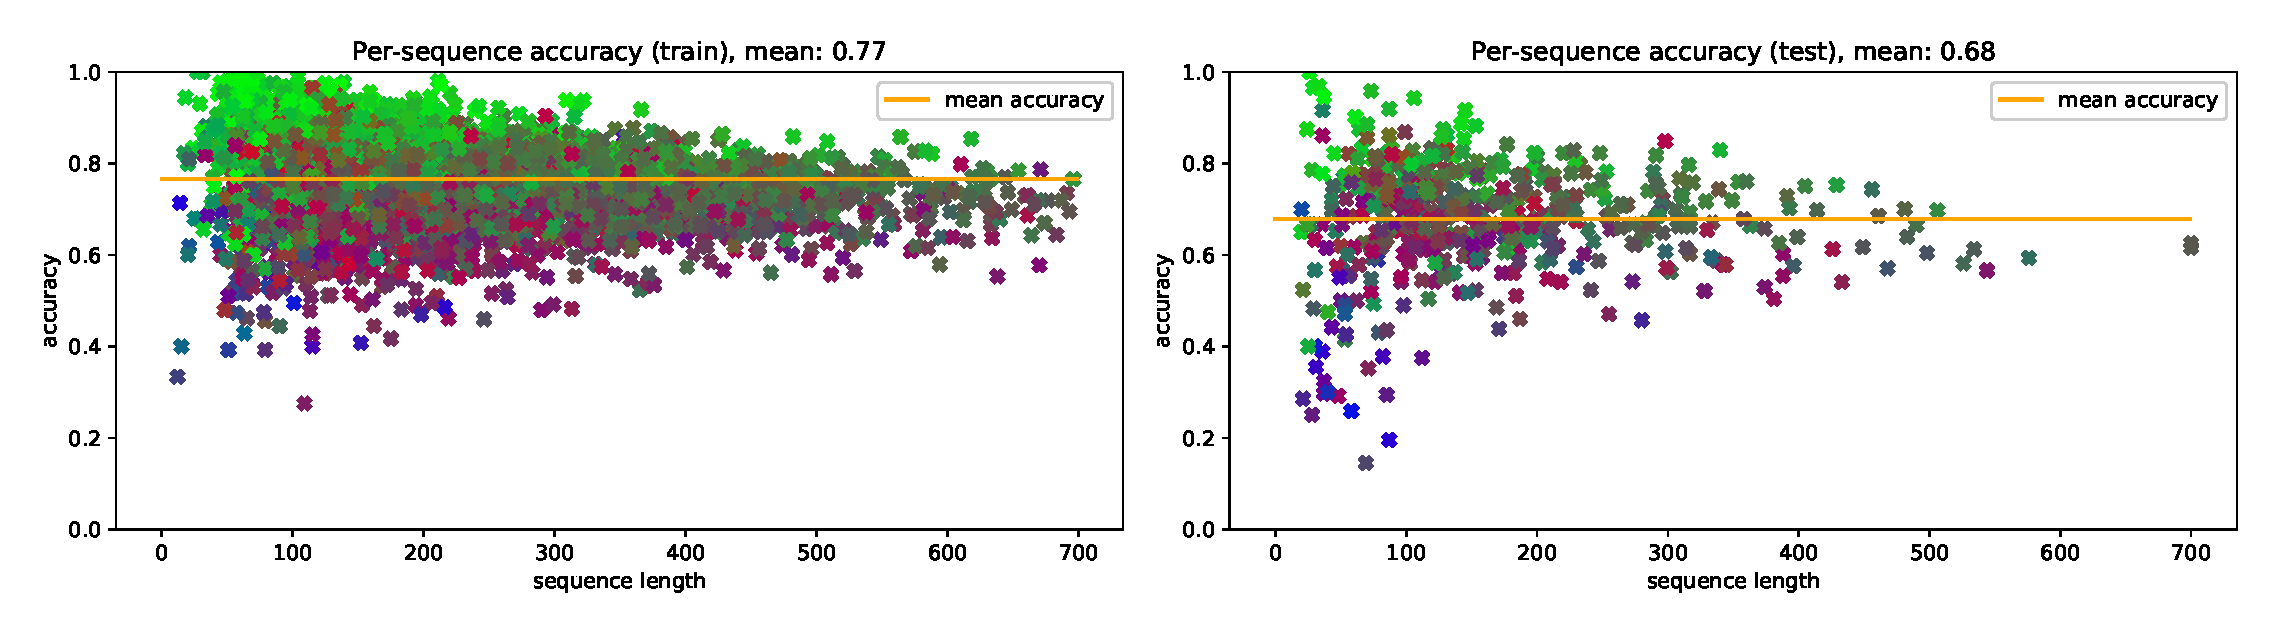
\includegraphics[width=1\linewidth]{Figures/per_seq_acc}
	\caption{\textit{The mean accuracy per sequence by sequence length.} The 5504 sequences of the training set are shown on the left and the 514 of the test set on the right. Each point represents a single protein, and its colour corresponds to the amount of $\beta$-sheets~(red), $\alpha$-helices (green), and coils (blue) it has. A purple point, for instance, would predominantly have $\beta$-sheets and coils.}
	\label{fig:per_seq_acc}
\end{figure}
% EXtra: include the same graph but colour the high-appearing classes and the low appearing classes differently (RB). Maybe not, in any case, some correlations plot

\section{Feature visualization}

\subsection{First layer filters}

\subsection*{Saliency maps on layers?}


\section{Saliency maps on inputs}

Before going through the analysis, it is worth recalling that the saliency map outputs has dimensions 8x42x19, for each position at each sequence, corresponding to the eight classes (outputs), the 42 inputs and the total window size of 19 (as explained in Section \ref{sect:saliency}).

%Talk about dimensions: saliency value, class, sequences, positions, window, amino-acids, aa/pssm (7 dimensions). From now on, individual saliency maps will refer to the saliency map of one sequence-position

\subsubsection*{Analysis on amino-acids and \textit{pssm}}
When looking at standard secondary-structure prediction algorithm, there is one point that may raise some suspicion: the inclusion of half of the inputs as one-hot encoded (amino-acids) and the other half as dense vectors (\textit{pssm}). One could think that this discrepancy may strongly favour the information coming from the dense part since the weights associated to it will learn much faster in a typical gradient descent learning schema.

Saliency maps can be used to prove whether this hypothesis is right by inspecting which of the input groups is being most decisive in the classification process. For doing so, each saliency map is divided into two groups of $8x21x19$, one corresponding to the values for one-hot amino-acids and the other for the \textit{pssm} inputs, and all the values inside each group are added up in absolute value to a single \textbf{saliency score}. Thus, each position of each sequence will have two scores, one for the amino-acids and one for the \textit{pssm}, and its comparison will give us which part of the inputs is more decisive and quantifies this difference. Only a single case out of the close to 1.3 million positions showed a higher one-hot than \textit{pssm} score and the difference only accounted for 1\% of their value. The rest of the scores were in favour of the \textit{pssm} saliency scores, with the distribution shown in Figure \ref{fig:aa_pssm}. From the figure, we can know that almost the totality of the \textit{pssm} scores were at least four times bigger than the one-hot ones, and therefore we can solidly confirm that the influence of the one-hot data on the input is minor and its omission would not cause much loss in the performance of the network. Consequently, further results focus only on the effect of the \textit{pssm} on classification.

\begin{figure}
	\centering
	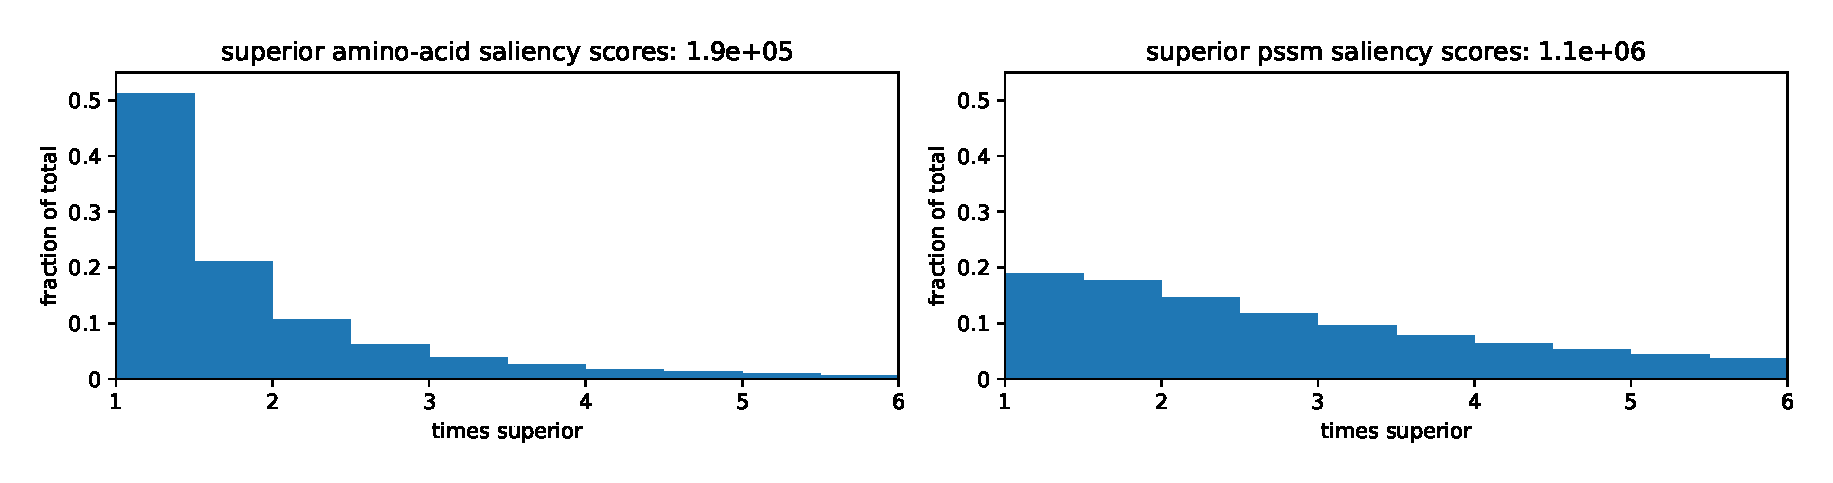
\includegraphics[width=1\linewidth]{Figures/aa_pssm}
	\caption{\textit{Pssm saliency superiority.} This figure shows a cumulative histogram of the number of positions whose \textit{pssm} saliency score was higher than the one-hot score. The $x$ axis represent the superiority ratio, i.e. how many times bigger was the score.}
	\label{fig:aa_pssm}
\end{figure}


%Options (all options could be applied either to aa or pssm, six dimensions left)

\subsection{Sequence-specific saliency maps}
This section will present the sort of analysis that can be done for a specific sequence. It can be especially useful for analysing the sequences whose accuracy was remarkably lower (outliers). Each sequence has a number of saliency maps equal to its length, $l$, and they can either be inspected one by one or be overlapped through the sequence, obtaining a single 8x42x$l$ \textbf{sequence map}.

% analyse per-class single sequence (sample-based) (4 dimensions left): aa-aggregated (3 dimensions) and added in the sequence position, either respecting each position (3 dimensions) or aggregating them in a heat map (2 dimensions), or aggregating the positions in a heat-map but containing the 8 classes (3 dimensions) (Colour the labels with the RGB either form Figure \ref{fig:per_seq_acc} or with the colour code from \ref{sect:sheer}).

%Have the x labels including amino-acid, prediction, and real label. Colour classes with the codes mentioned in the previous paragraph. Consider marking mismatches in bold.

Figure \ref{fig:sliding} shows consecutive saliency maps belonging to a single class. The patterns they present are generally preserved (note the differences in scales), just being shifted by one position on the window axis. It suggests that the algorithm is not differentiating that much between specific amino-acid positions, but instead looking for them to be in the vicinity. For this reason, we can consider that overlapping them in a single sequence map does preserve most of the information, as it is shown in Figure \ref{fig:sample_8classes}. This sort of map reveals which amino-acids of the vicinity are mostly responsible for a prediction in a particular position. For instance, the predictions of class \textit{E} on the left side of the shown fragment have to do with the presence of amino-acids \textit{A}, \textit{V} and \textit{L}, while the failure to predict class \textit{H} on position 109 is likely related to the presence of amino-acid \textit{D} at position 110. Note that these saliency values come from the aggregation of all the 42 inputs and not only from the one-hot encoded side, which explains why positions 105 and 106 have different values despite having the same amino-acid (\textit{D}). It is especially important to take this into account since we have discussed before that one-hot amino-acid information is not as decisive for making the predictions.

Another issue worth noting is a non-realistic inconsistency among predictions: the algorithm assigns labels individually per-position and does not take into account the labels it is providing at the sides. It leads to situations such as having individual \textit{G}s when these only come at least in groups of three. Different approaches in the state-of-the-art for dealing with this are adding a \textit{struct2struct} machine on top of the predictions~\cite{Rost1993,Fang2017}, iterative processes that learn from previous step's prediction~\cite{Heffernan2017}, or probabilistic methods that convey information about adjacent positions, like \textit{Conditional random fields}~\cite{Wang2016} or \textit{next-step conditioning}~\cite{Busia2017}.

For a more in-depth look into the whole \textit{pssm} spectrum, we would need to narrow the scope down to a single class, as it is done in Figure \ref{fig:sample_Hclass}. This figure reveals that is indeed common that the real amino-acid in the sequence is not among the most influential ones from the \textit{pssm} for making the decision. Note that the pssm values of the amino-acids do not always need to have contributions of the same sign (such as \textit{P} or \textit{D} in the figure), revealing that the network is capturing something more than a pure presence: location and combinations of amino acids are also prominent.

\begin{figure}
	\centering
	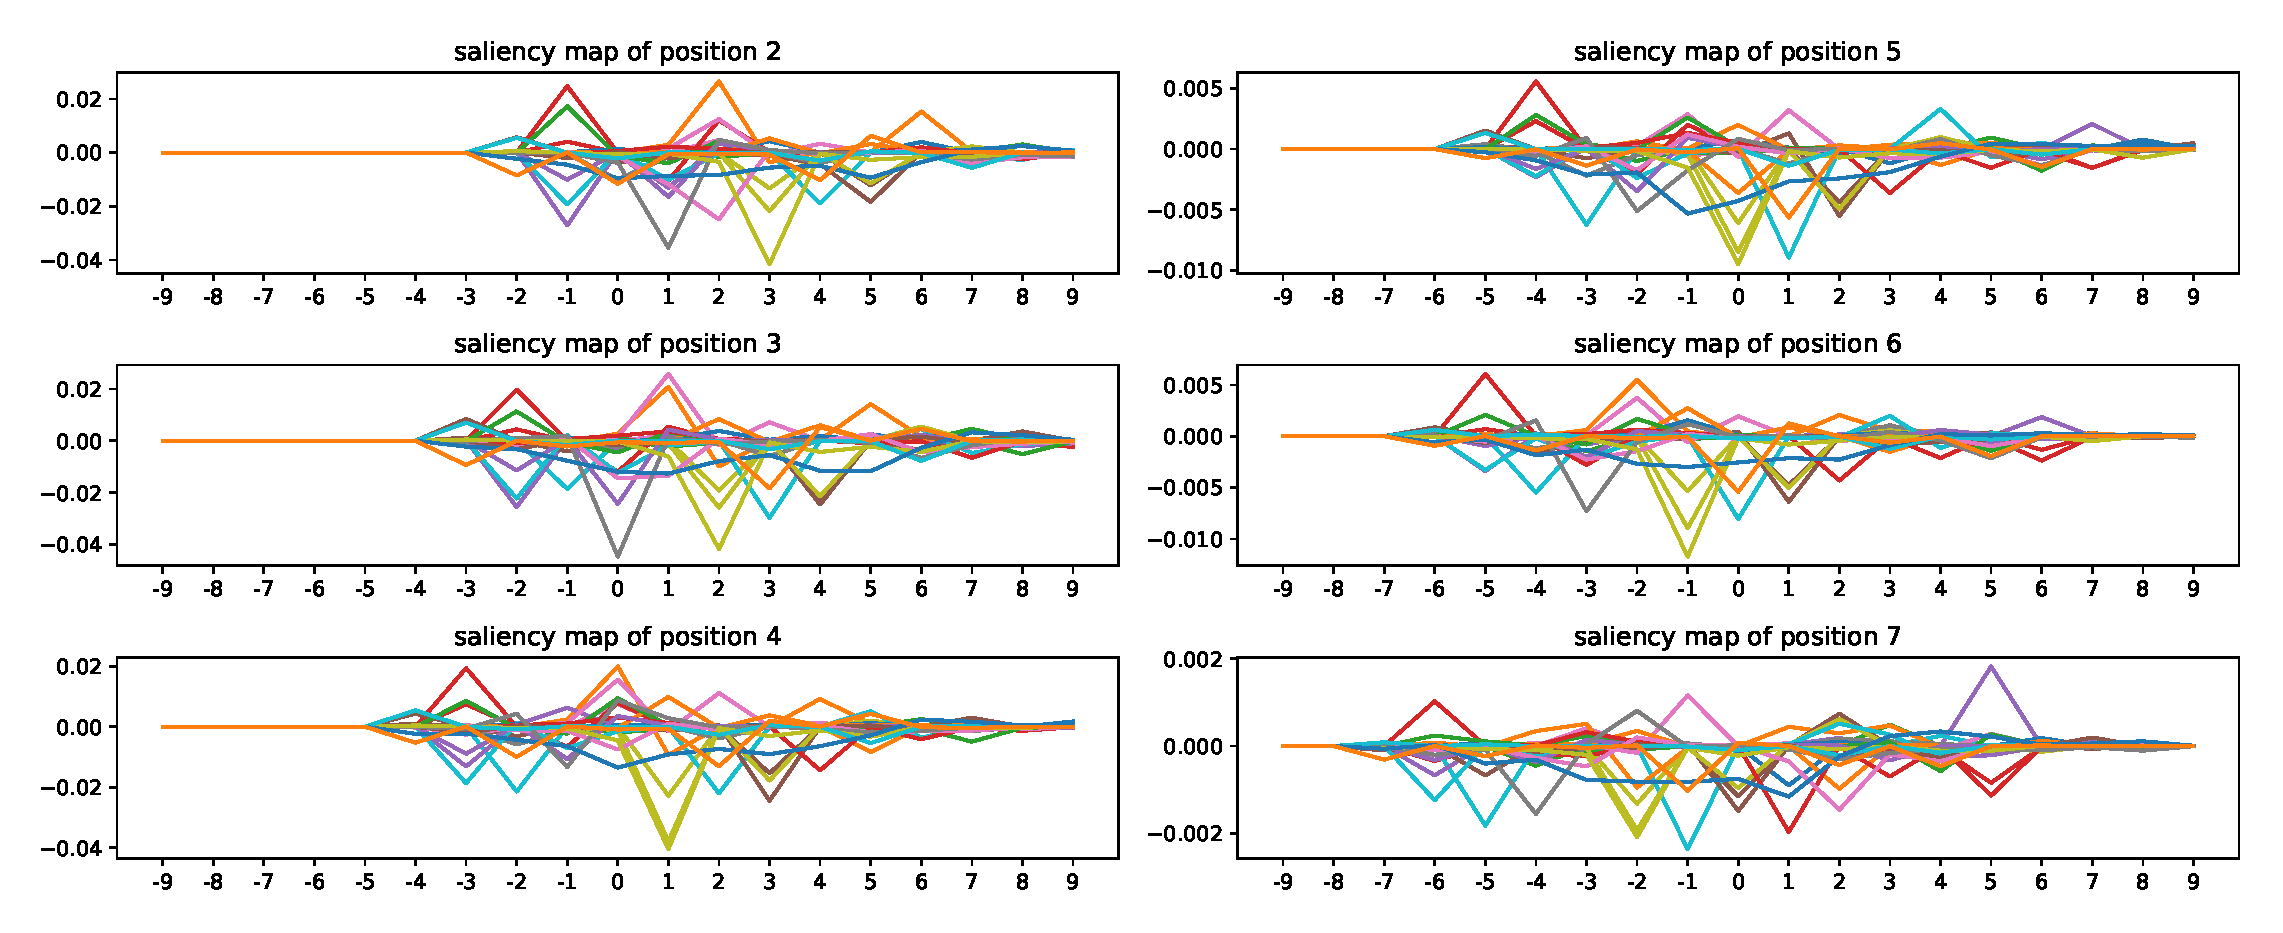
\includegraphics[width=1\linewidth]{Figures/sliding}
	\caption{\textit{Saliency maps for consecutive positions in a sequence.} In every sub-figure there are 42 lines of the 42 inputs, corresponding to their saliency values for class \textit{H}.}
	\label{fig:sliding}
\end{figure}


\begin{figure}
	\centering
	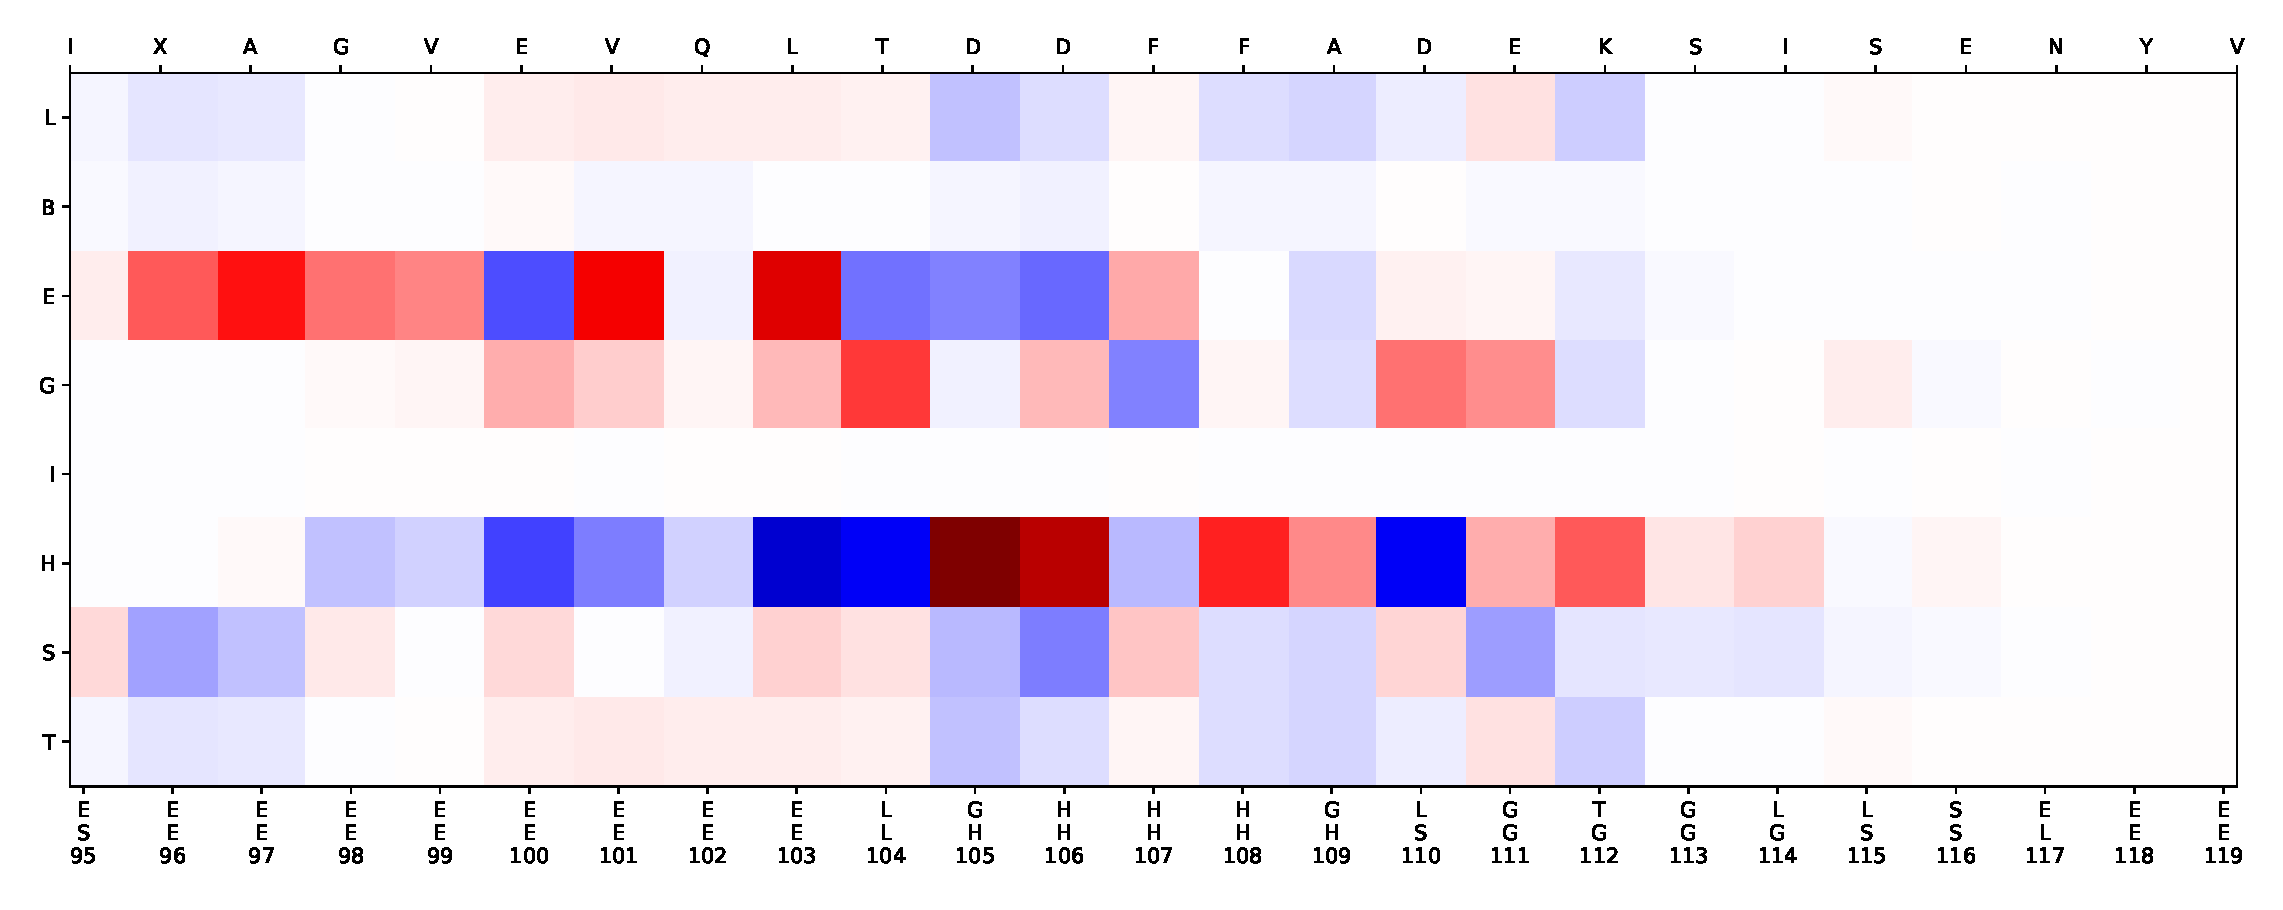
\includegraphics[width=1\linewidth]{Figures/sample_8classes}
	\caption{\textit{Fragment of a sequence map aggregated by the input.} Each line corresponds to the aggregated saliency values of one of the eight output classes. The upper $x$ axis displays the amino-acids in the sequence. The lower $x$ axis contains three sets of labels in this order: the predictions, the true values, and the positions in the sequence. The code of colours of the labels is the same as the lines and is set according to the class of the predictions.}
	\label{fig:sample_8classes}
\end{figure}

\begin{figure}
	\centering
	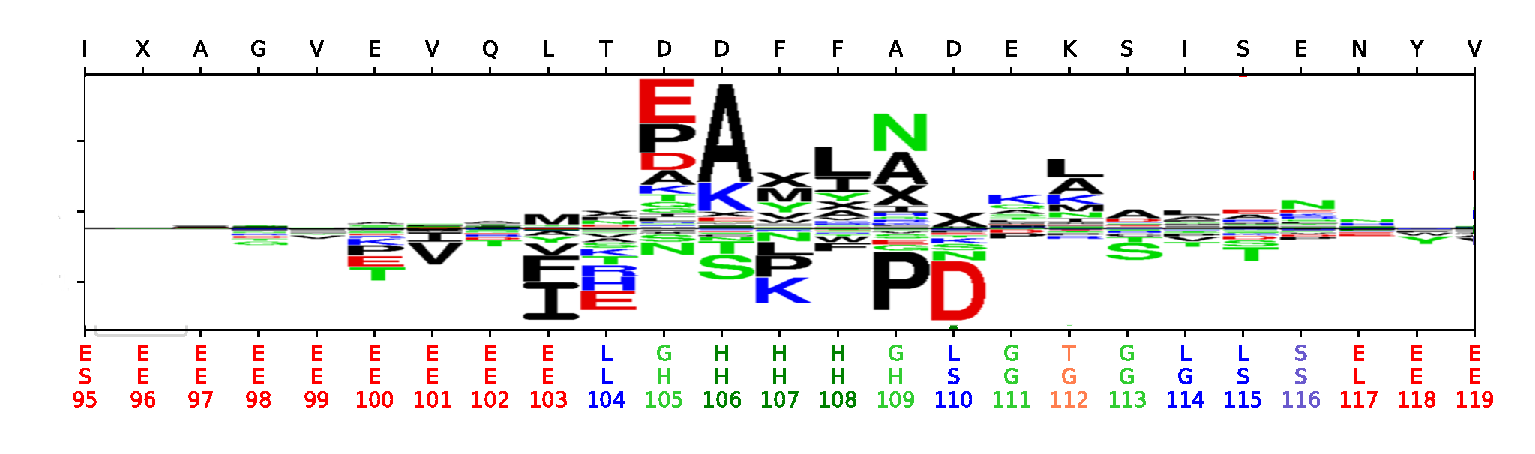
\includegraphics[width=1\linewidth]{Figures/sample_Hclass}
	\caption{\textit{Fragment of sequence map for class H in SeqLogo form.} The saliency of the \textit{pssm} values is shown here. The frame and labels of the figure is the same as in Figure \ref{fig:sample_8classes}. The image has been generated by \textit{SeqLogo} \cite{Thomsen2012}.}
	\label{fig:sample_Hclass}
\end{figure}


% HAve as the sample one of the sequences with low accuracy and high length from \ref{sect:outliers}?

\subsection{Class-specific and pssm-specific saliency maps}
Instead of looking at the saliency information along single sequences, aggregating the information from all the 1.3 million saliency maps could give us some broader information of what the network has learned. Again, the high dimensionality of the data to explore requires us to seek meaningful ways to aggregate and represent the data.

\subsubsection*{Sheer addition} \label{sect:sheer}
A simple way to aggregate the saliency maps would be adding them up with element-wise addition, thus composing a single saliency map of size 8x42x19. This mega-saliency map should convey rough information of the general features of the network. Since there is no a sense of ``left" or ``right" in the sequences, the aggregation should be \textit{side-invariant} and therefore an extra \textit{mirroring} operation is applied to the aggregation in order to make the aggregated saliency map symmetric along the centre of the window.

To start with, Figure \ref{fig:class_agg_class} shows the aggregated class-specific saliency maps for the three main classes and the 21 \textit{pssm} values. There are a few details to notice here. First, higher saliency values concentrate around the centre of the window, meaning that most relevant information is located around five positions from the predicted one. Second, most \textit{pssm} values preserve the same sign along the window of a class, although a few exceptions also occur. Third, as it could be expected, class \textit{L} generally presents inverse patterns with respect to classes \textit{H} and \textit{E}. It makes sense since coils appear wherever there are no $\alpha$-helices or $\beta$-strands, they are complementary. Lastly, each class has a ``feature" \textit{pssm} value that is their best indicator: \textit{A} for class \textit{H}; \textit{V} for \textit{E}; and \textit{P} for \textit{L}.

\begin{figure}
	\centering
	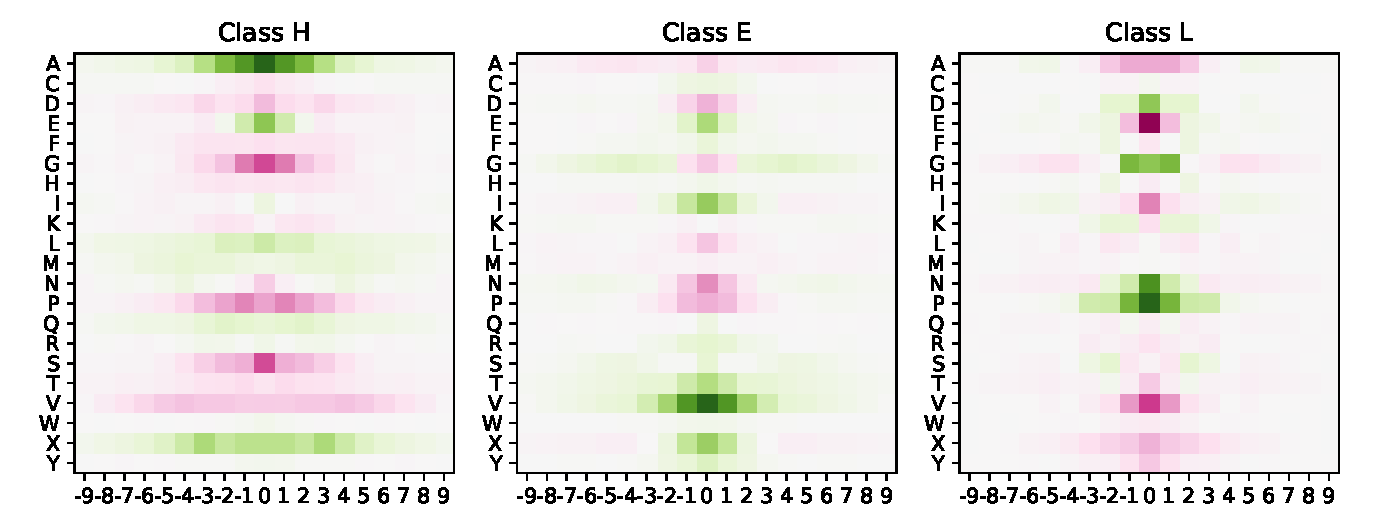
\includegraphics[width=1\linewidth]{Figures/class_agg_class}
	\caption{\textit{Per-class aggregated saliency maps of the main three classes along the window.} Only the saliency values of \textit{pssm} are shown here. Green means positive saliency values and purple means negative.}
	\label{fig:class_agg_class}
\end{figure}

Figure \ref{fig:class_agg_aa} shows the same information but from a different perspective: as it is \textit{pssm-specific}, it focuses on how a single \textit{pssm}'s position affects the classification on the eight classes. These plots show important effects of the position, as all of them make significant shifts at the centre of the window. \textit{Pssm} value \textit{G} strongly favours coils at its spot, but foresees the presence of $\beta$-strands a few positions away. \textit{Pssm} value \textit{K} has somehow similar behaviour, although with a more intricate ladder of classes while moving further away from the centre. \textit{Pssm} value \textit{M} is generally favouring $\alpha$-helices, although $3_{10}$-helices gain equal importance at the very centre. Note the difference in scales, which indicates that \textit{pssm}-values of \textit{G} are in any case more influential than the other two.

\begin{figure}
	\centering
	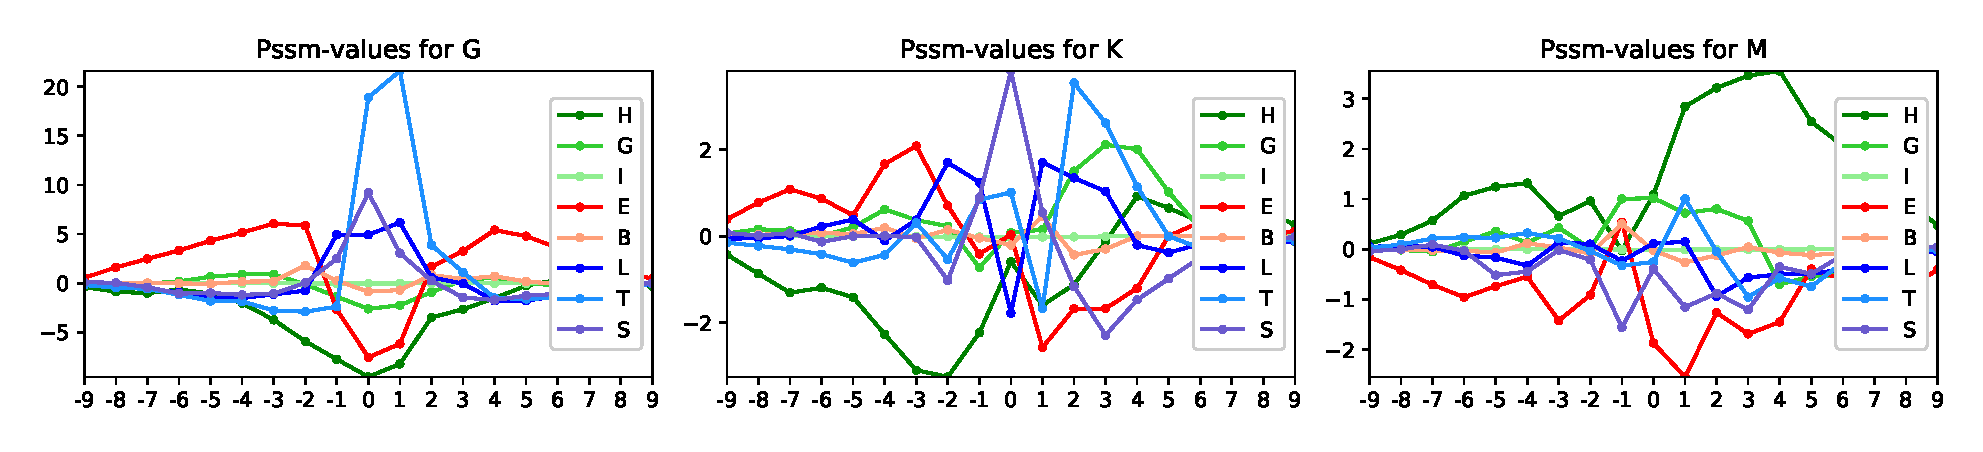
\includegraphics[width=1\linewidth]{Figures/class_agg_aa}
	\caption{\textit{Per-class aggregated saliency map of amino-acids G, K, and M, in this order.} \textit{Y} axis is in 1000s. Note the change in scale, particularly for the left-most plot~(amino-acid \textit{G}).}
	\label{fig:class_agg_aa}
\end{figure}

We can use the aggregated saliency maps to investigate the span of the class influence, i.e. how much of the further away positions the network uses to predict the class. For performing this analysis, the addition of the saliency maps must be done in absolute value and then aggregated by the \textit{pssm} dimension as well. Figure \ref{fig:sheer_class_aa} reveals the results for this operation. $\alpha$-helices (\textit{H}) and $\beta$-bridges (\textit{B}) seem to have the highest side influence, although $\beta$-strand's \textit{E} influence gets more weight for further positions. Most classes show a quasi-linear descend on influence from one to five-positions away and some tail afterwards. Coils are the most centred classes.

\begin{figure}
	\centering
	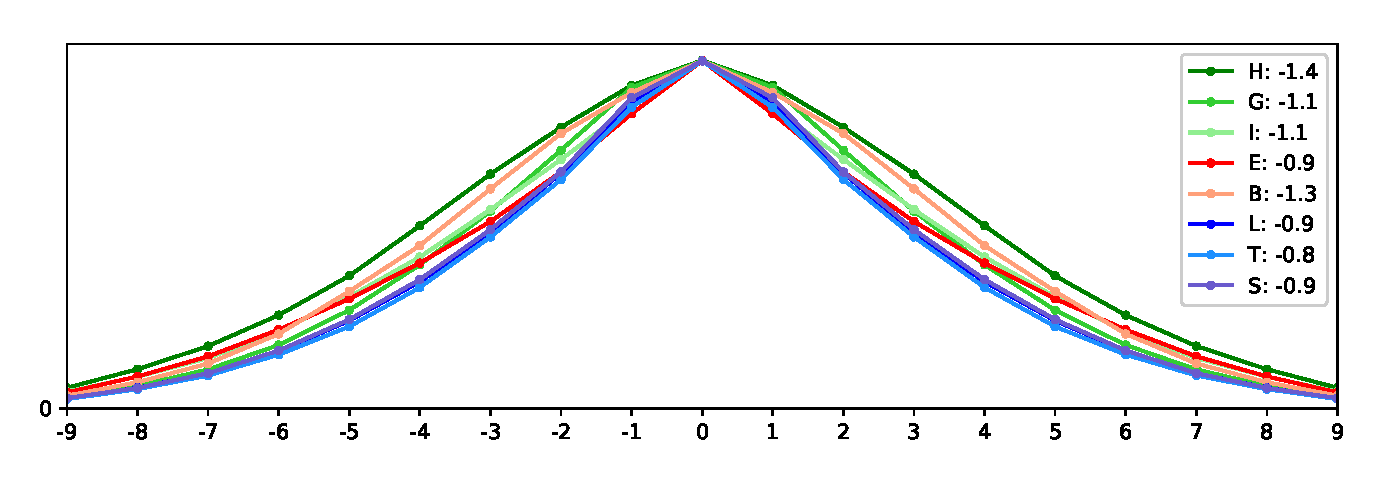
\includegraphics[width=1\linewidth]{Figures/sheer_class_aa}
	\caption{\textit{Classes overall influence along the window size.} All lines are normalized to have the same hight , as the analysis focuses on the shapes rather than the values. Labels include a measurement of the \textit{kurtosis} of the distributions.}
	\label{fig:sheer_class_aa}
\end{figure}


% SHould I try to compare my results with known motifs? Absolutely yes!

\subsubsection*{Clustering techniques}
Aggregate all individual saliency maps % SHould I try to compare my results with known motifs? Absolutely yes!
%clustering (5 dimensions left)
%Using the per-class window-aggregated version of individual saliency maps (4 dimensions left)
%Cosine distance metric.
%Show either all profiles per-cluster (3 dimensions) or aggregated profiles (2 dimensions)
%Show t-SNE with points coloured by cluster

\begin{figure}
	\centering
	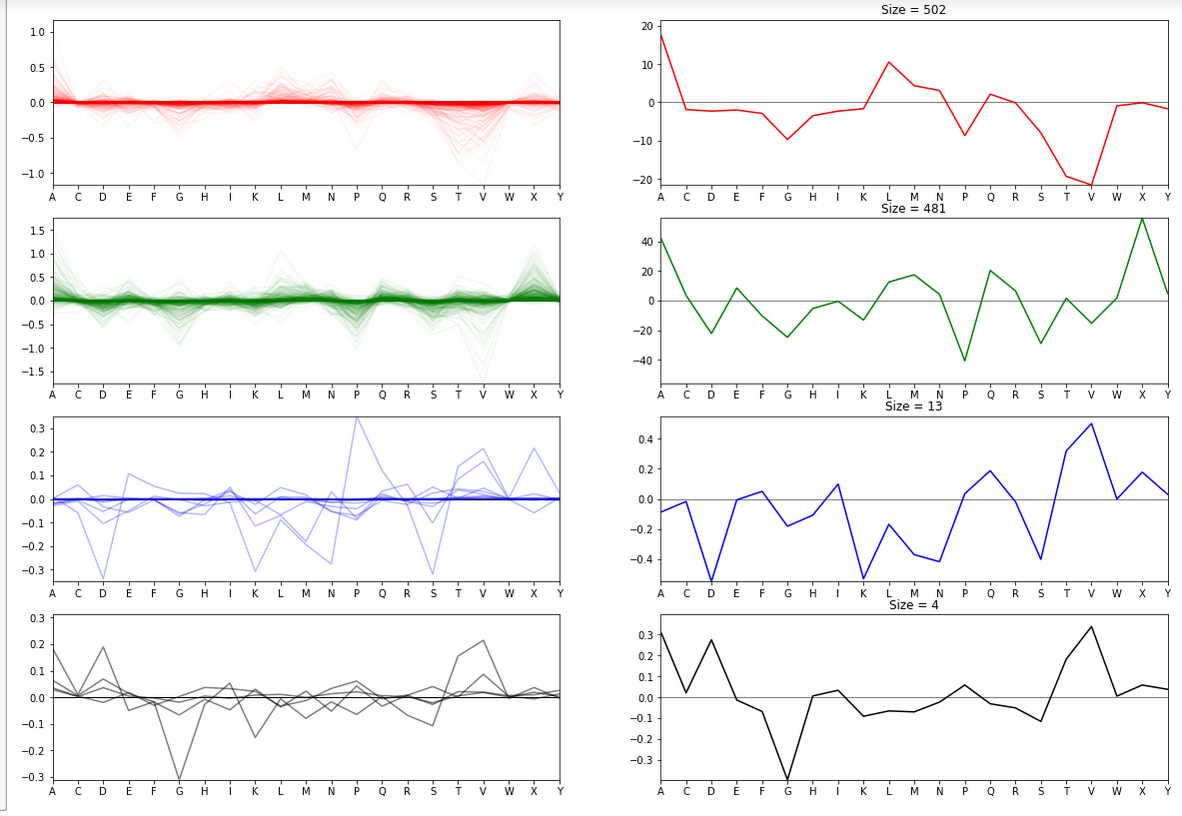
\includegraphics[width=1\linewidth]{Figures/clusters}
	\caption{}
	\label{fig:clusters}
\end{figure}

\begin{figure}
	\centering
	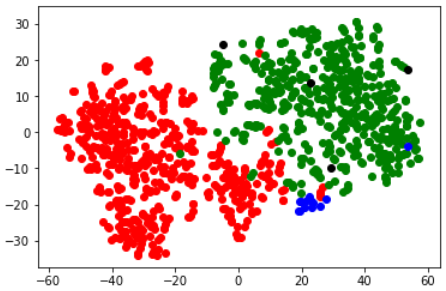
\includegraphics[width=0.7\linewidth]{tsne}
	\caption{}
	\label{fig:tsne}
\end{figure}


\section{Final discussion and future research}
%INclude rest of graphs in appendix A
The results shown here are a small sub-sample of the kind of information that can be obtained from saliency maps. An exhaustive catalogue including plots for all classes and \textit{pssm} values can be found in Appendix \ref{Chapter:App}.

Section \ref{sect:saliency} introduced the state-of-the-art techniques for saliency maps. This work has applied the gradient * input approach, as it leverage well simplicity and effectiveness. Although more recent techniques for calculating saliency maps proved to have better results and they should be applied in further research, the whole framework for aggregating and evaluating them still holds and is independent of how the saliency maps were calculated.

The choice of protein secondary structure prediction is rooted in that it is a well-known problem. There has been some discussion on whether it is the best middle-step for reaching 3D structures, based on the fact that classification of secondary structure in these eight types has some degree of arbitrariness. The main alternative is predicting the angles of the backbone between every two amino-acids, transforming the problem from classification to regression. While translating the techniques developed here to this new problem is not straightforward, big parts of it ---as the ideas for aggregating saliency maps--- can be recycled and adapted to the new context.

% SHouldn't types of errors have different costs? It is as bad to miss a Q8 prediction that was in the same Q3 prediction class